\documentclass[border=2pt]{standalone}
\usepackage{amsmath,amssymb}
\usepackage{tikz}
\usetikzlibrary{positioning,arrows.meta,calc}
\begin{document}
\fontsize{10}{12}\selectfont
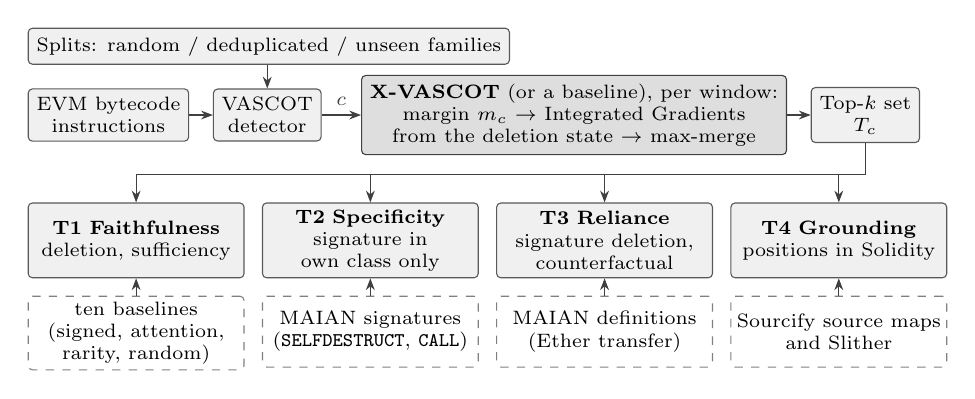
\begin{tikzpicture}[font=\scriptsize, >={Stealth[length=1.5mm]},
  box/.style={draw=black!65, rounded corners=1.5pt, align=center, inner sep=3pt, fill=black!6},
  xv/.style={draw=black!75, rounded corners=1.5pt, align=center, inner sep=3pt, fill=black!13},
  test/.style={draw=black!65, rounded corners=1.5pt, align=center, inner sep=2pt, fill=black!6, text width=26mm, minimum height=9.5mm, execute at begin node={\hyphenpenalty=10000\relax}},
  ref/.style={draw=black!50, dashed, rounded corners=1.5pt, align=center, inner sep=2pt, fill=white, text width=26mm, minimum height=9mm, execute at begin node={\hyphenpenalty=10000\relax}},
  arr/.style={->, black!75}]
\node[box] (in) {EVM bytecode\\ instructions};
\node[box, right=3mm of in] (det) {VASCOT\\ detector};
\node[xv, right=5mm of det] (xv) {\textbf{X-VASCOT} (or a baseline), per window:\\
  margin $m_c$ $\rightarrow$ Integrated Gradients\\ from the deletion state $\rightarrow$ max-merge};
\node[box, right=3mm of xv] (topk) {Top-$k$ set\\ $T_c$};
\node[box, above=3mm of in.north west, anchor=south west] (split) {Splits: random / deduplicated / unseen families};
\draw[arr] (in) -- (det);
\draw[arr] (det) -- node[above]{$c$} (xv);
\draw[arr] (xv) -- (topk);
\draw[arr] (split.south -| det.north) -- (det.north);
\node[test, anchor=north west] (t1) at ($(in.west |- xv.south)+(0,-6mm)$) {\textbf{T1 Faithfulness}\\ deletion, sufficiency};
\node[test, right=2.2mm of t1] (t2) {\textbf{T2 Specificity}\\ signature in own class only};
\node[test, right=2.2mm of t2] (t3) {\textbf{T3 Reliance}\\ signature deletion, counterfactual};
\node[test, right=2.2mm of t3] (t4) {\textbf{T4 Grounding}\\ positions in Solidity};
\node[ref, below=2.2mm of t1] (r1) {ten baselines (signed, attention, rarity, random)};
\node[ref, below=2.2mm of t2] (r2) {MAIAN signatures\\ (\texttt{SELFDESTRUCT}, \texttt{CALL})};
\node[ref, below=2.2mm of t3] (r3) {MAIAN definitions\\ (Ether transfer)};
\node[ref, below=2.2mm of t4] (r4) {Sourcify source maps\\ and Slither};
\foreach \a/\b in {r1/t1,r2/t2,r3/t3,r4/t4} \draw[arr] (\a) -- (\b);
\coordinate (bus) at ($(t1.north)+(0,3.5mm)$);
\draw[black!75] (topk.south) -- (topk.south |- bus);
\draw[black!75] (t1.north |- bus) -- (t4.north |- bus) -- (topk.south |- bus);
\foreach \t in {t1,t2,t3,t4} \draw[arr] (\t.north |- bus) -- (\t.north);
\end{tikzpicture}
\end{document}
